
%\documentclass[a4paper,11pt,twoside]{ThesisStyle}
\documentclass[a4paper,11pt,twoside]{article}

\date{\today}
\usepackage{amsmath,amssymb}             % AMS Math
% \usepackage[french]{babel}
\usepackage[latin1]{inputenc}
\usepackage[OT1]{fontenc}
\usepackage[left=2.7cm,right=1.7cm,top=1.6cm,bottom=1.6cm,includefoot,includehead,headheight=13.6pt]{geometry}
\usepackage{setspace}
\usepackage{epigraph}
\usepackage{lineno}


%\usepackage{arev}
%\usepackage[bitstream-charter]{mathdesign}
%\usepackage[urw-garamond]{mathdesign}
%\usepackage[sfmath]{kpfonts} %% sfmath option only to make math in sans serif. Probablye only for use when base font is sans serif.
%\renewcommand*\familydefault{\sfdefault} %% Only if the base font of the document is to be sans serif
\usepackage[sc]{mathpazo}
\linespread{1.05}   
\usepackage[T1]{fontenc}



% Table of contents for each chapter

\usepackage[nottoc, notlof, notlot]{tocbibind}
\usepackage{minitoc}
\setcounter{minitocdepth}{2}
\mtcindent=15pt
% Use \minitoc where to put a table of contents

\usepackage{aecompl}

% Glossary / list of abbreviations

\usepackage[intoc]{nomencl}
\renewcommand{\nomname}{List of Abbreviations}

\makenomenclature

% My pdf code

\usepackage{graphicx,type1cm,eso-pic,color}
\usepackage{lscape}

  \usepackage[pagebackref,hyperindex=true]{hyperref}

%\geometry{letterpaper}
%\graphicspath{{.}{images/}}

% nicer backref links
\renewcommand*{\backref}[1]{}
\renewcommand*{\backrefalt}[4]{%
\ifcase #1 %
(Not cited.)%
\or
(Cited on page~#2.)%
\else
(Cited on pages~#2.)%
\fi}
\renewcommand*{\backrefsep}{, }
\renewcommand*{\backreftwosep}{ and~}
\renewcommand*{\backreflastsep}{ and~}

% Links in pdf
\usepackage{color}
\definecolor{linkcol}{rgb}{0,0,0.4} 
\definecolor{citecol}{rgb}{0.5,0,0} 

% Change this to change the informations included in the pdf file

% See hyperref documentation for information on those parameters

\hypersetup
{
bookmarksopen=true,
pdftitle="",
pdfauthor="", pdfsubject="", %subject of the document
%pdftoolbar=false, % toolbar hidden
pdfmenubar=true, %menubar shown
pdfhighlight=/O, %effect of clicking on a link
colorlinks=true, %couleurs sur les liens hypertextes
pdfpagemode=None, %aucun mode de page
pdfpagelayout=SinglePage, %ouverture en simple page
pdffitwindow=true, %pages ouvertes entierement dans toute la fenetre
linkcolor=linkcol, %couleur des liens hypertextes internes
citecolor=citecol, %couleur des liens pour les citations
urlcolor=linkcol %couleur des liens pour les url
}

% definitions.
% -------------------

\setcounter{secnumdepth}{3}
\setcounter{tocdepth}{2}

% Some useful commands and shortcut for maths:  partial derivative and stuff
\newcommand{\xbp}{$x_{Bj}$}
\newcommand{\xb}{$x_{Bj}~$}
\newcommand{\ptp}{$p_\perp^2$}
\newcommand{\pt}{$p_\perp^2~$}
\newcommand{\dptp}{$\Delta \langle p_\perp^2 \rangle$}
\newcommand{\dpt}{$\Delta \langle p_\perp^2 \rangle ~$}

\brokenpenalty10000\relax

\newcommand{\pd}[2]{\frac{\partial #1}{\partial #2}}
\def\abs{\operatorname{abs}}
\def\argmax{\operatornamewithlimits{arg\,max}}
\def\argmin{\operatornamewithlimits{arg\,min}}
\def\diag{\operatorname{Diag}}
\newcommand{\eqRef}[1]{(\ref{#1})}

\usepackage{rotating}                    % Sideways of figures & tables
%\usepackage{bibunits}
%\usepackage[sectionbib]{chapterbib}          % Cross-reference package (Natural BiB)
%\usepackage{natbib}                  % Put References at the end of each chapter
                                         % Do not put 'sectionbib' option here.
                                         % Sectionbib option in 'natbib' will do.
\usepackage{fancyhdr}                    % Fancy Header and Footer

% \usepackage{txfonts}                     % Public Times New Roman text & math font
  
%%% Fancy Header %%%%%%%%%%%%%%%%%%%%%%%%%%%%%%%%%%%%%%%%%%%%%%%%%%%%%%%%%%%%%%%%%%
% Fancy Header Style Options

\pagestyle{fancy}                       % Sets fancy header and footer
\fancyfoot{}                            % Delete current footer settings

%\renewcommand{\chaptermark}[1]{         % Lower Case Chapter marker style
%  \markboth{\chaptername\ \thechapter.\ #1}}{}} %

%\renewcommand{\sectionmark}[1]{         % Lower case Section marker style
%  \markright{\thesection.\ #1}}         %

\fancyhead[LE,RO]{\bfseries\thepage}    % Page number (boldface) in left on even
% pages and right on odd pages
\fancyhead[RE]{\bfseries\nouppercase{\leftmark}}      % Chapter in the right on even pages
\fancyhead[LO]{\bfseries\nouppercase{\rightmark}}     % Section in the left on odd pages

\let\headruleORIG\headrule
\renewcommand{\headrule}{\color{black} \headruleORIG}
\renewcommand{\headrulewidth}{1.0pt}
\usepackage{colortbl}
\arrayrulecolor{black}

\fancypagestyle{plain}{
  \fancyhead{}
  \fancyfoot{}
  \renewcommand{\headrulewidth}{0pt}
}

%\usepackage{algorithm}
%\usepackage[noend]{algorithmic}

%%% Clear Header %%%%%%%%%%%%%%%%%%%%%%%%%%%%%%%%%%%%%%%%%%%%%%%%%%%%%%%%%%%%%%%%%%
% Clear Header Style on the Last Empty Odd pages
\makeatletter

\def\cleardoublepage{\clearpage\if@twoside \ifodd\c@page\else%
  \hbox{}%
  \thispagestyle{empty}%              % Empty header styles
  \newpage%
  \if@twocolumn\hbox{}\newpage\fi\fi\fi}

\makeatother
 
%%%%%%%%%%%%%%%%%%%%%%%%%%%%%%%%%%%%%%%%%%%%%%%%%%%%%%%%%%%%%%%%%%%%%%%%%%%%%%% 
% Prints your review date and 'Draft Version' (From Josullvn, CS, CMU)
\newcommand{\reviewtimetoday}[2]{\special{!userdict begin
    /bop-hook{gsave 20 710 translate 45 rotate 0.8 setgray
      /Times-Roman findfont 12 scalefont setfont 0 0   moveto (#1) show
      0 -12 moveto (#2) show grestore}def end}}
% You can turn on or off this option.
% \reviewtimetoday{\today}{Draft Version}
%%%%%%%%%%%%%%%%%%%%%%%%%%%%%%%%%%%%%%%%%%%%%%%%%%%%%%%%%%%%%%%%%%%%%%%%%%%%%%% 

\newenvironment{maxime}[1]
{
\vspace*{0cm}
\hfill
\begin{minipage}{0.5\textwidth}%
%\rule[0.5ex]{\textwidth}{0.1mm}\\%
\hrulefill $\:$ {\bf #1}\\
%\vspace*{-0.25cm}
\it 
}%
{%

\hrulefill
\vspace*{0.5cm}%
\end{minipage}
}

\let\minitocORIG\minitoc
\renewcommand{\minitoc}{\minitocORIG \vspace{1.5em}}

\usepackage{multirow}
%\usepackage{slashbox}

\newenvironment{bulletList}%
{ \begin{list}%
	{$\bullet$}%
	{\setlength{\labelwidth}{25pt}%
	 \setlength{\leftmargin}{30pt}%
	 \setlength{\itemsep}{\parsep}}}%
{ \end{list} }

\newtheorem{definition}{D�finition}
\renewcommand{\epsilon}{\varepsilon}

% centered page environment

\newenvironment{vcenterpage}
{\newpage\vspace*{\fill}\thispagestyle{empty}\renewcommand{\headrulewidth}{0pt}}
{\vspace*{\fill}}


\begin{document}

\title{\centering{Investigating the Fermi motion effects on the incoherent DVCS 
channel}}
\maketitle

In our DVCS analysis, we considered the initial proton of the incoherent 
channel to be at rest, while this is not totally true because of the Fermi 
motion. Does this assumption is a good approximation? what other options can be 
used to minimize this effect on the calculated exclusive quantities?\\

Figure \ref{fig:handbag} presents the leading order handbag diagram of the 
incoherent DVCS channel off $^4$He, where the nucleus breaks and the DVCS 
occurs on a bound nucleon. Ideally, the transferred momentum squared ($t$) is 
defined using the initial and the final nucleons' 4-vectors as $(p-p')^{2}$.  
Then as a DVCS requirement, $t$ has to be greater than a certain value 
($t_{min}$), that is defined using the kinematics of the incoming and the 
scattered electrons. Due to the knowledge lack of the initial proton's 
momentum, this cut maybe inaccurate causes loosing some good DVCS events. In 
this work, we try to tackle this issue and check the stability of the 
reconstructed beam-spin asymmetry, as being our DVCS observable.\\ 

\begin{figure}[h!]
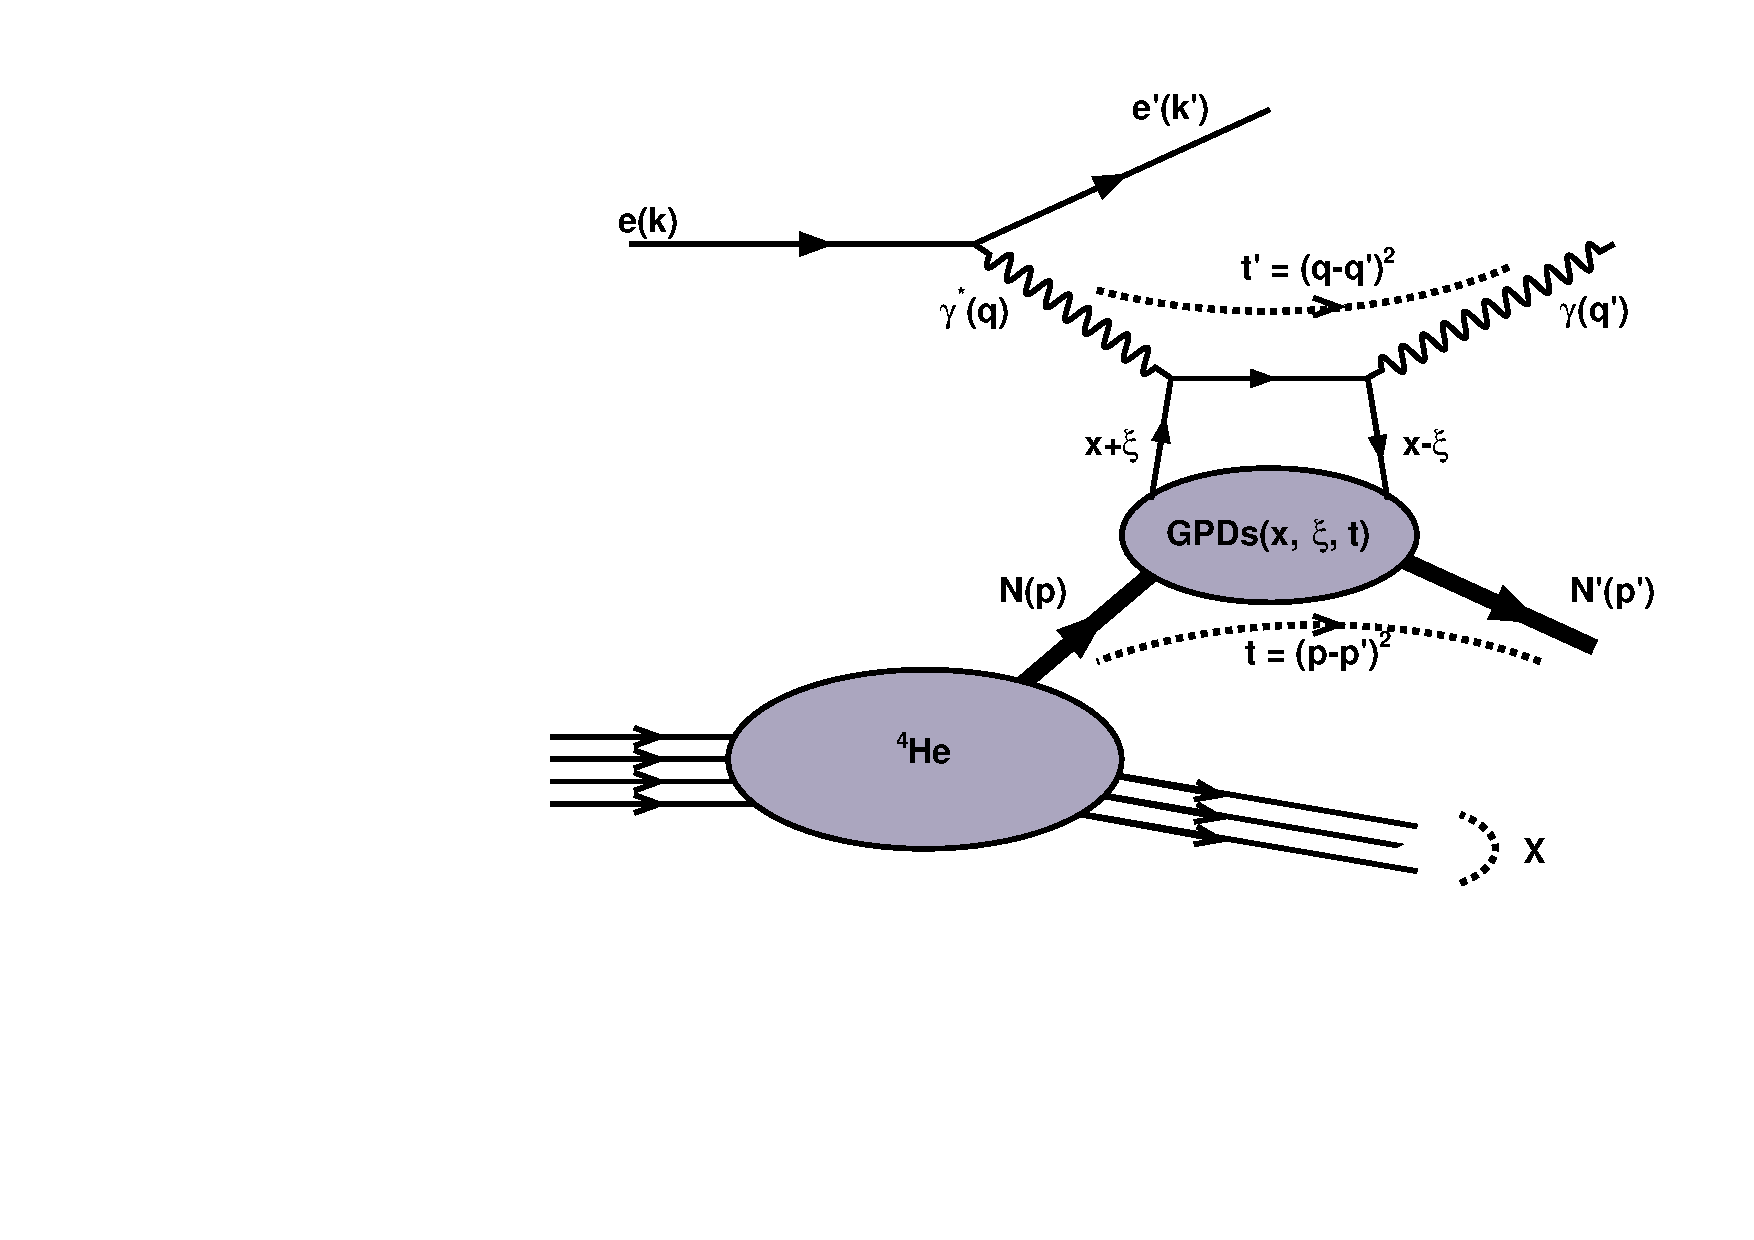
\includegraphics[height=10.0cm]{fig/handbag_incoherent.pdf}
\caption{Representation of the leading order handbag diagram of the incoherent 
DVCS process off $^4$He}
\label{fig:handbag}
\end{figure}

Typically, the transferred momentum squared $t$ is equal to the transferred 
momentum squared ($t'$) defined between the virtual photon and the final-state 
real photon, as shown in Figure \ref{fig:handbag}.  While defining the momentum 
transferred as $t'$ is a good way to pass the Fermi motion effect on the 
initial bound proton, it is more smeared than than $t$ due to bigger energy 
resolutions of the photons. Figure \ref{fig:tprime} shows the distributions of 
the coherent and the incoherent relative difference between $t$ and $t'$. One 
can see that the coherent DVCS channel, the distributions is symmetric and 
centered at zero as expected due to our good knowledge on the initial $^4$He 
target, while it is not exactly the case for the incoherent case due to the 
Fermi motion.\\            

\begin{figure}[h!]
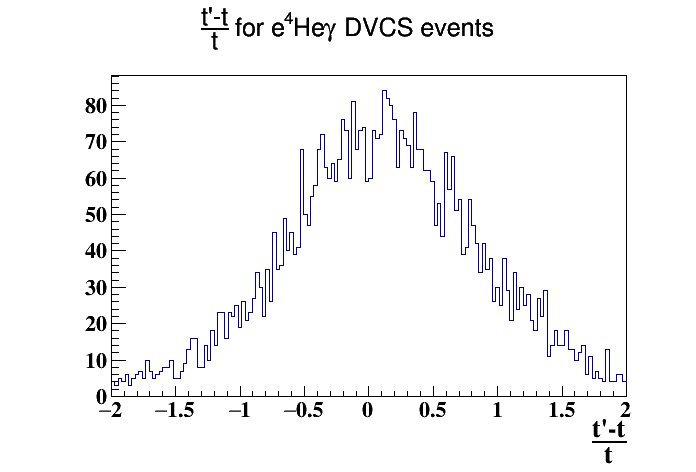
\includegraphics[height=5.0cm]{fig/T_tprime_Coh.png}
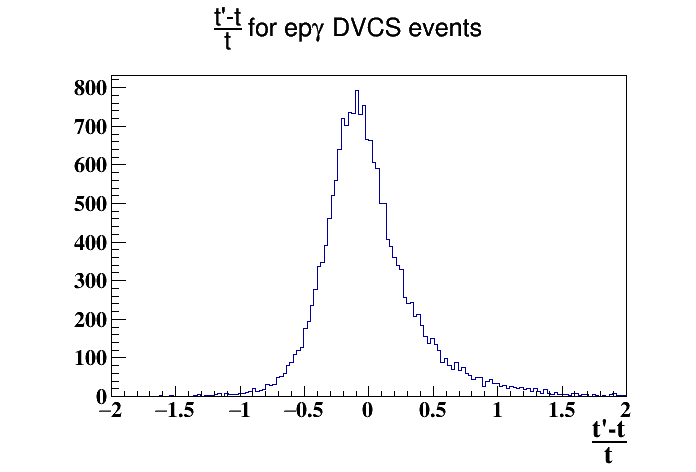
\includegraphics[height=5.0cm]{fig/T_tprime_InCoh.png}
\caption{On the left: the coherent relative difference between $t$ and $t'$.  
On the right: the incoherent relative difference.}
\label{fig:tprime}
\end{figure}

In the following, we check the effects of defining the transferred momentum 
squared as $t$ and $t'$ on the exclusive distributions and on the reconstructed 
beam-spin asymmetries. Figure \ref{fig:cuts_t} presents the exclusive 
distributions of the incoherent DVCS events where the transferred momentum
squared is defined as $t$, while it is define as $t'$ in figure 
\ref{fig:cuts_tprime}. To minimize the smearing effects of $t'$ on the 
exclusive distributions, 2$\sigma$ exclusive cuts were optimized compared to 
3$\sigma$ cuts which were applied in the $t$ case. In terms of collected 
statistics, the 2$\sigma$ cuts using $t'$ gave almost the same statistics using 
$t$. From comparing the exclusive distributions, especially the $ep\gamma$ 
missing energy and the missing mass squared, one sees that using $t'$ gives 
more Gaussian missing energy distributions and cleaner missing mass squared 
distribution.\\      

\begin{figure}[h!]
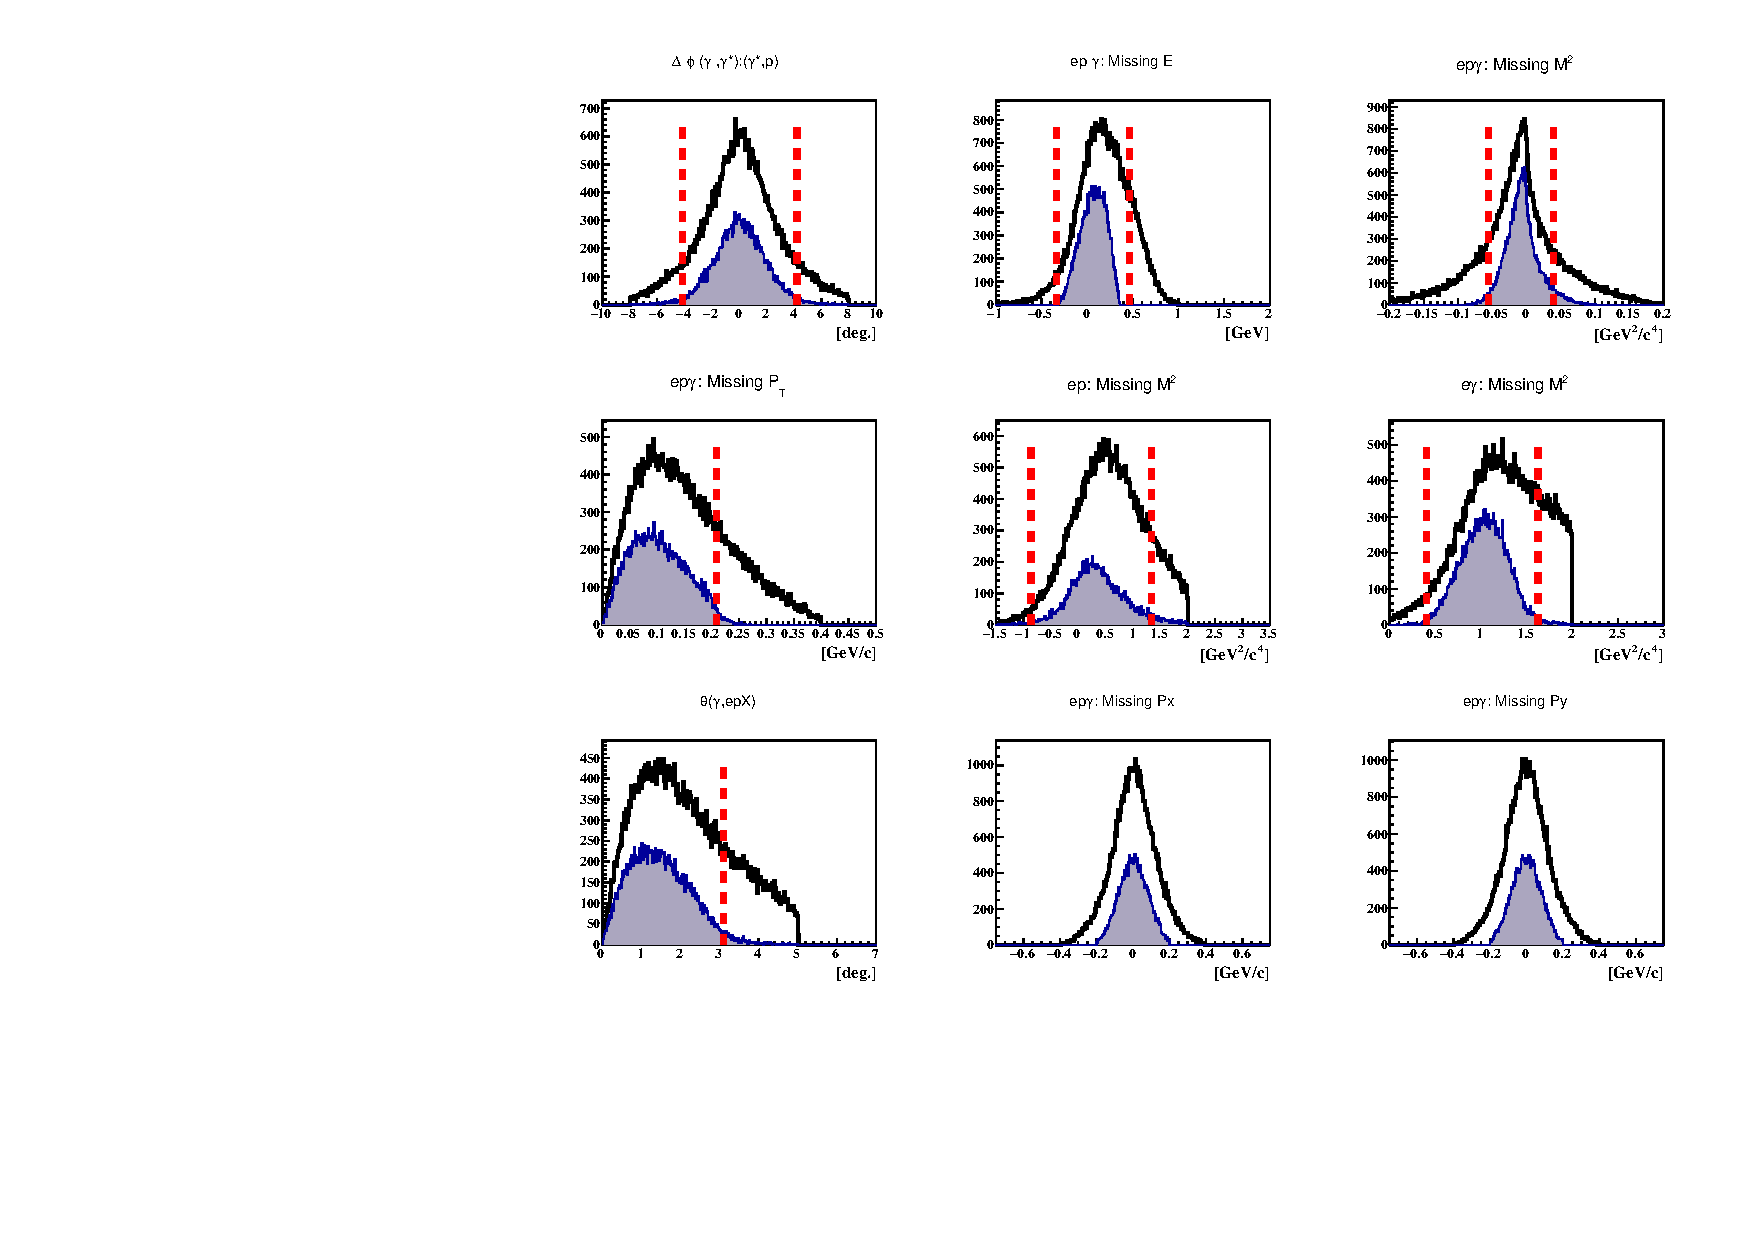
\includegraphics[height=15.0cm]{fig/old_all_incoh_exc_cuts.pdf}
\caption{The old set of exclusive cuts with $t$>$t_{min}$. The black
   distributions represent the incoherent DVCS events candidate. The shaded
   distributions represent the events which passed all the exclusivity cuts
   except the quantity plotted. The vertical red lines represent the applied
exclusivity, 3$\sigma$ cuts.}
\label{fig:cuts_t}
\end{figure}

\begin{figure}[h!]
   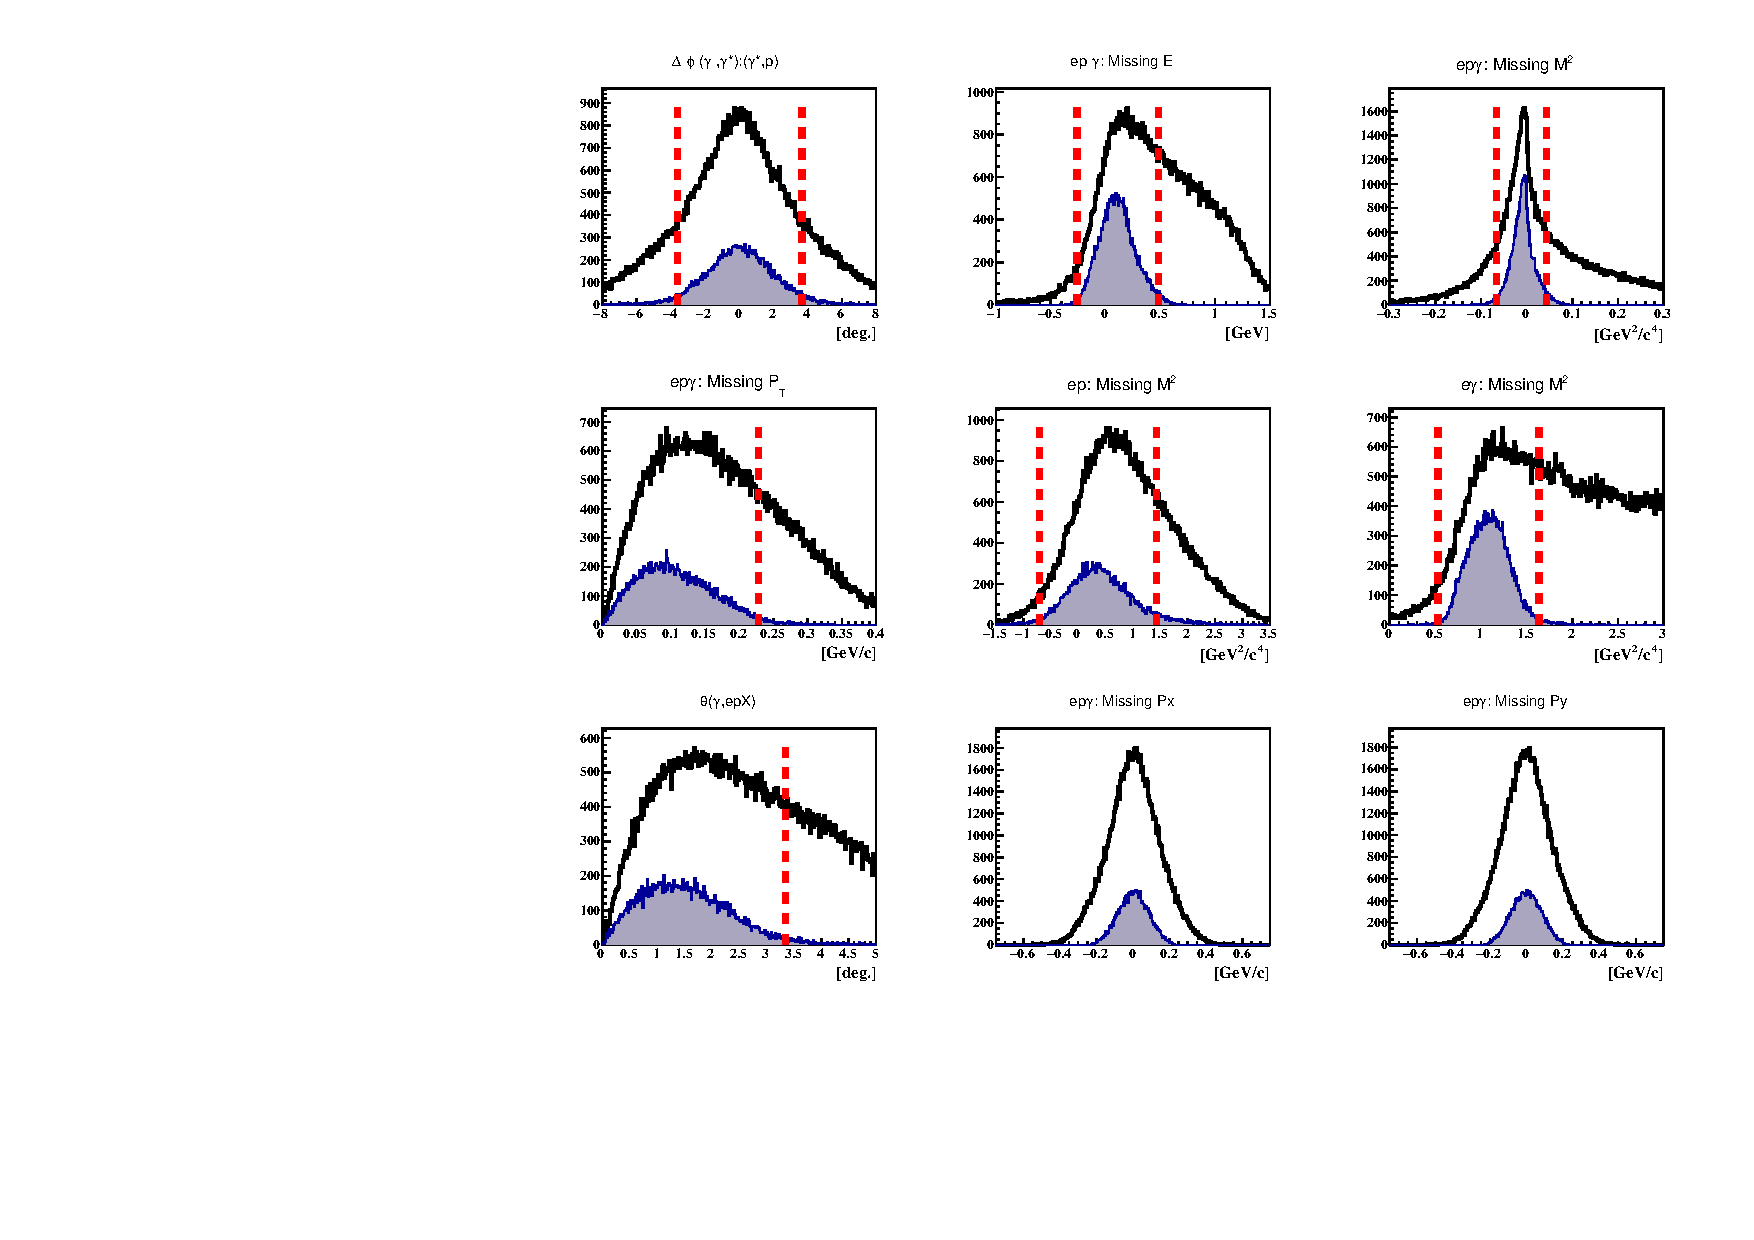
\includegraphics[height=15.0cm]{fig/all_incoh_exc_cuts_test.pdf}
   \caption{New set of exclusive cuts with $t'$>$t_{min}$. The black
      distributions represent the incoherent DVCS events candidate. The shaded
      distributions represent the events which passed all the exclusivity cuts
      except the quantity plotted. The vertical red lines represent the applied 
   exclusivity, 2$\sigma$ cuts.}
\label{fig:cuts_tprime}
\end{figure}

Figure \ref{fig:bsa_incoh_bins} shows our measured incoherent beam-spin
asymmetries, for the three sets of the two-dimensional bins, in the two 
scinarios of defining the transferred momentum squared. The $Q^2$, $x_{B}$, and 
$-t$-dependencies of $A_{LU}$ at $\phi$=~90$^{\circ}$ (the $\alpha$ parameter 
of the fit) are shown in figure \ref{fig:incoh_Q2_xB_t_ALU}.



\begin{figure}[h!]
   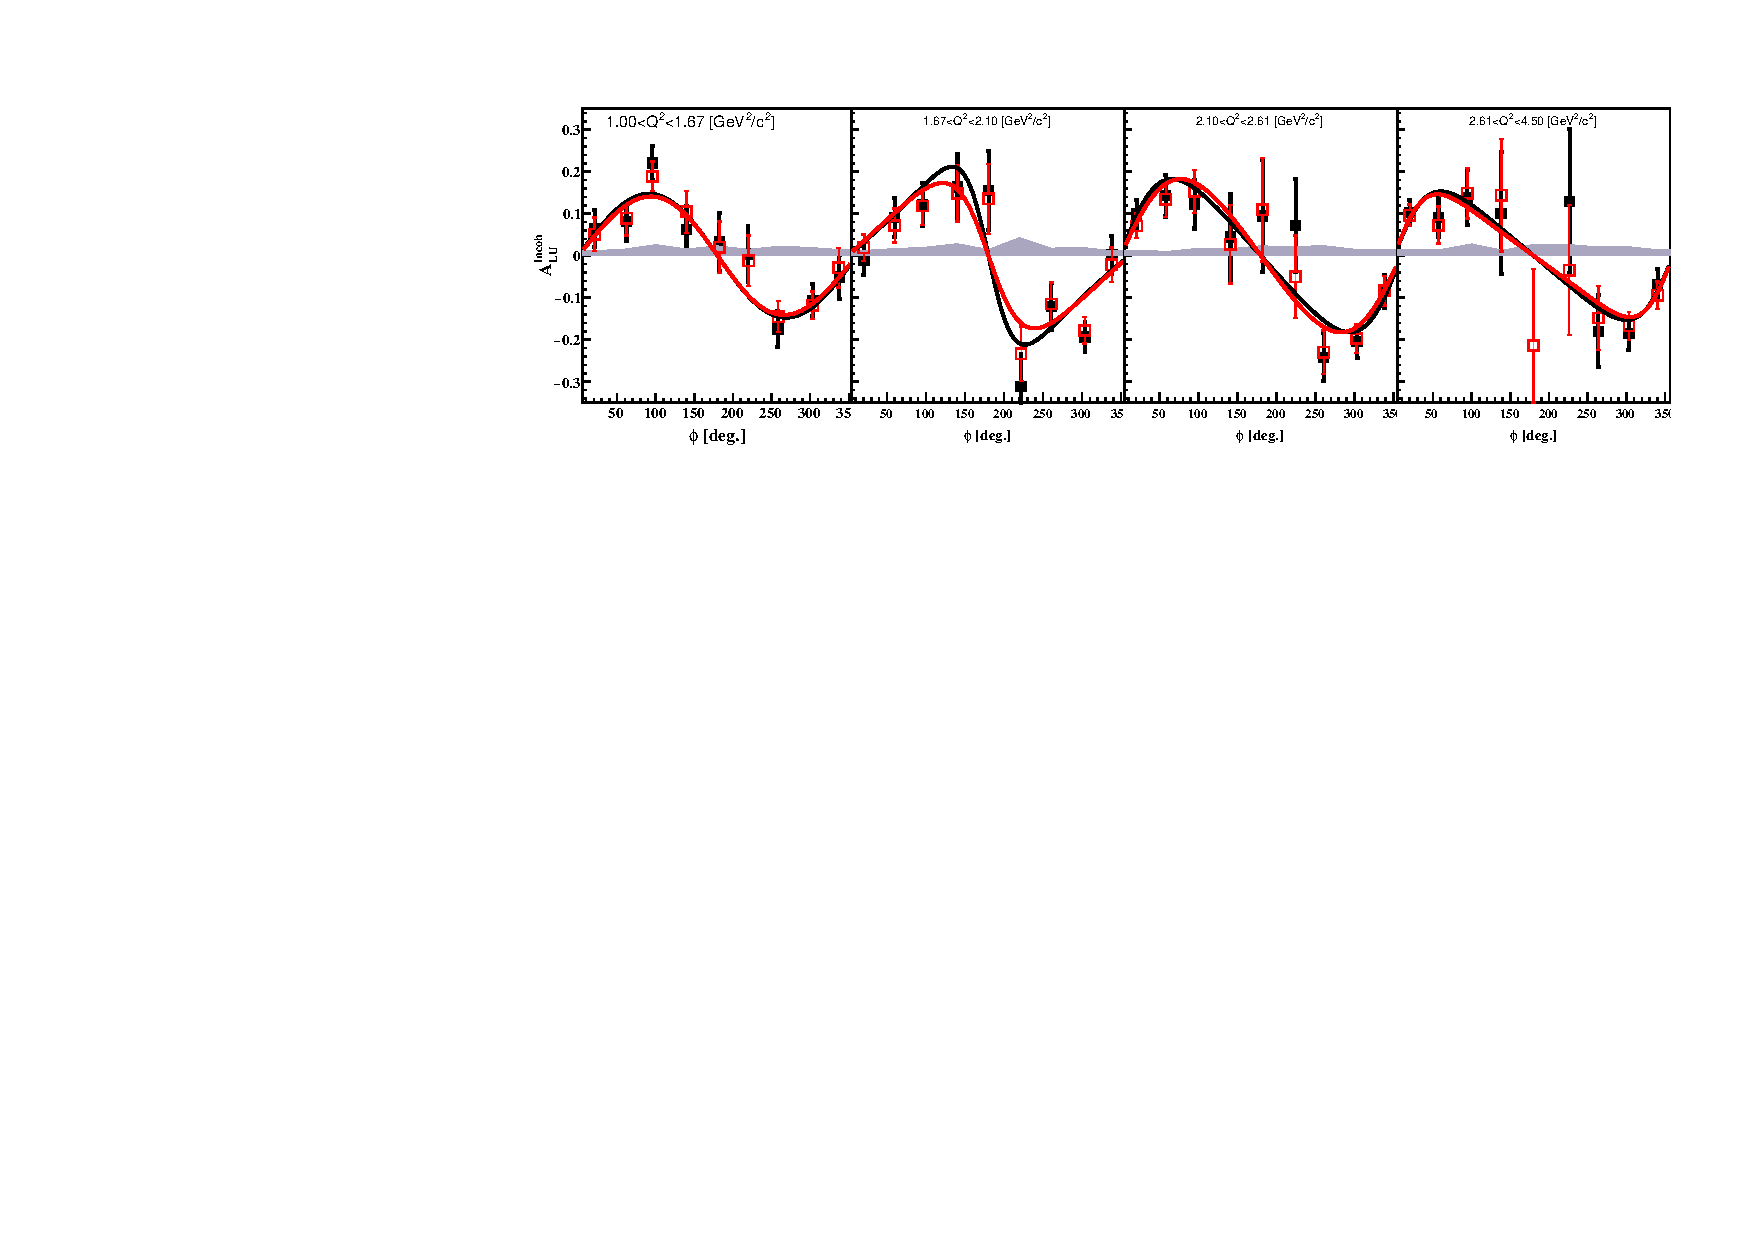
\includegraphics[height=6.0cm]{fig/ALU_phi_p_Q2.pdf}
   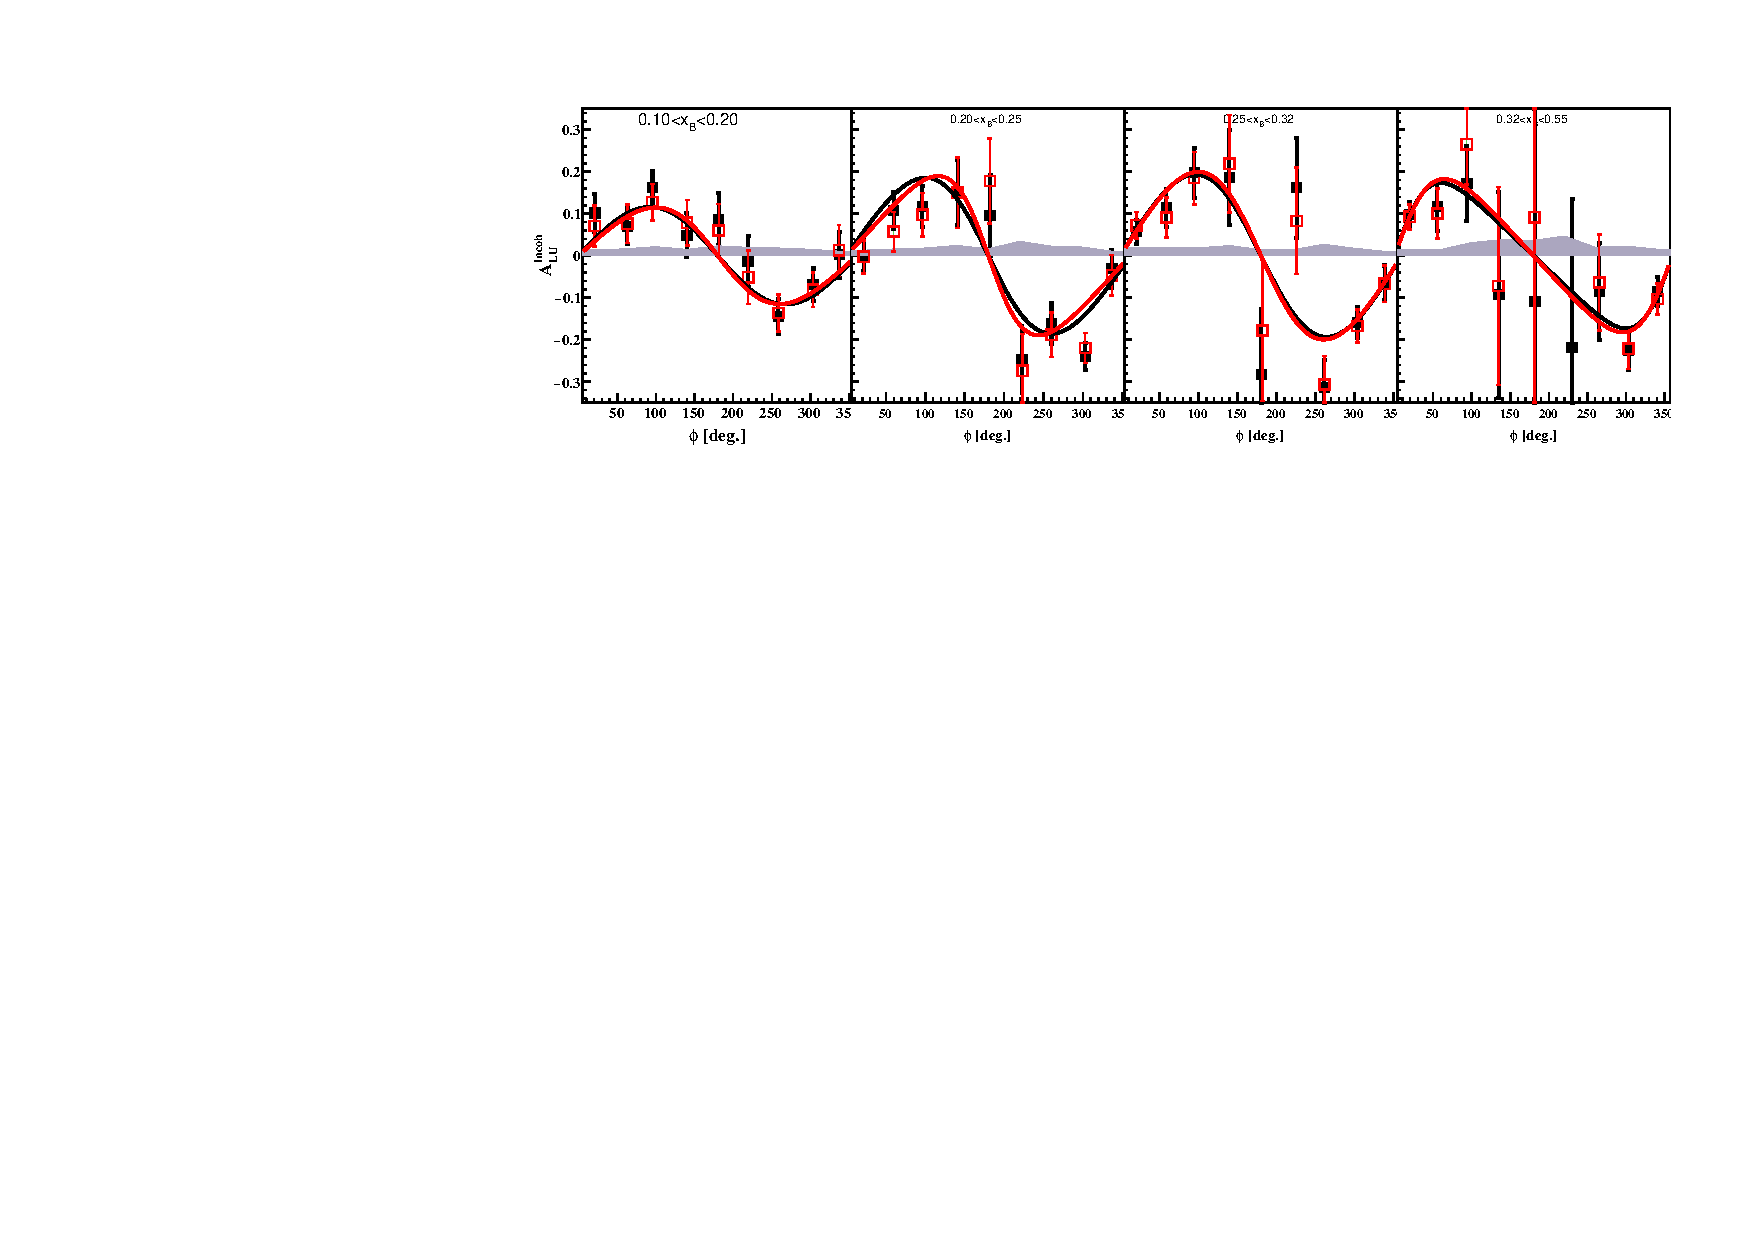
\includegraphics[height=6.0cm]{fig/ALU_phi_p_x.pdf}
   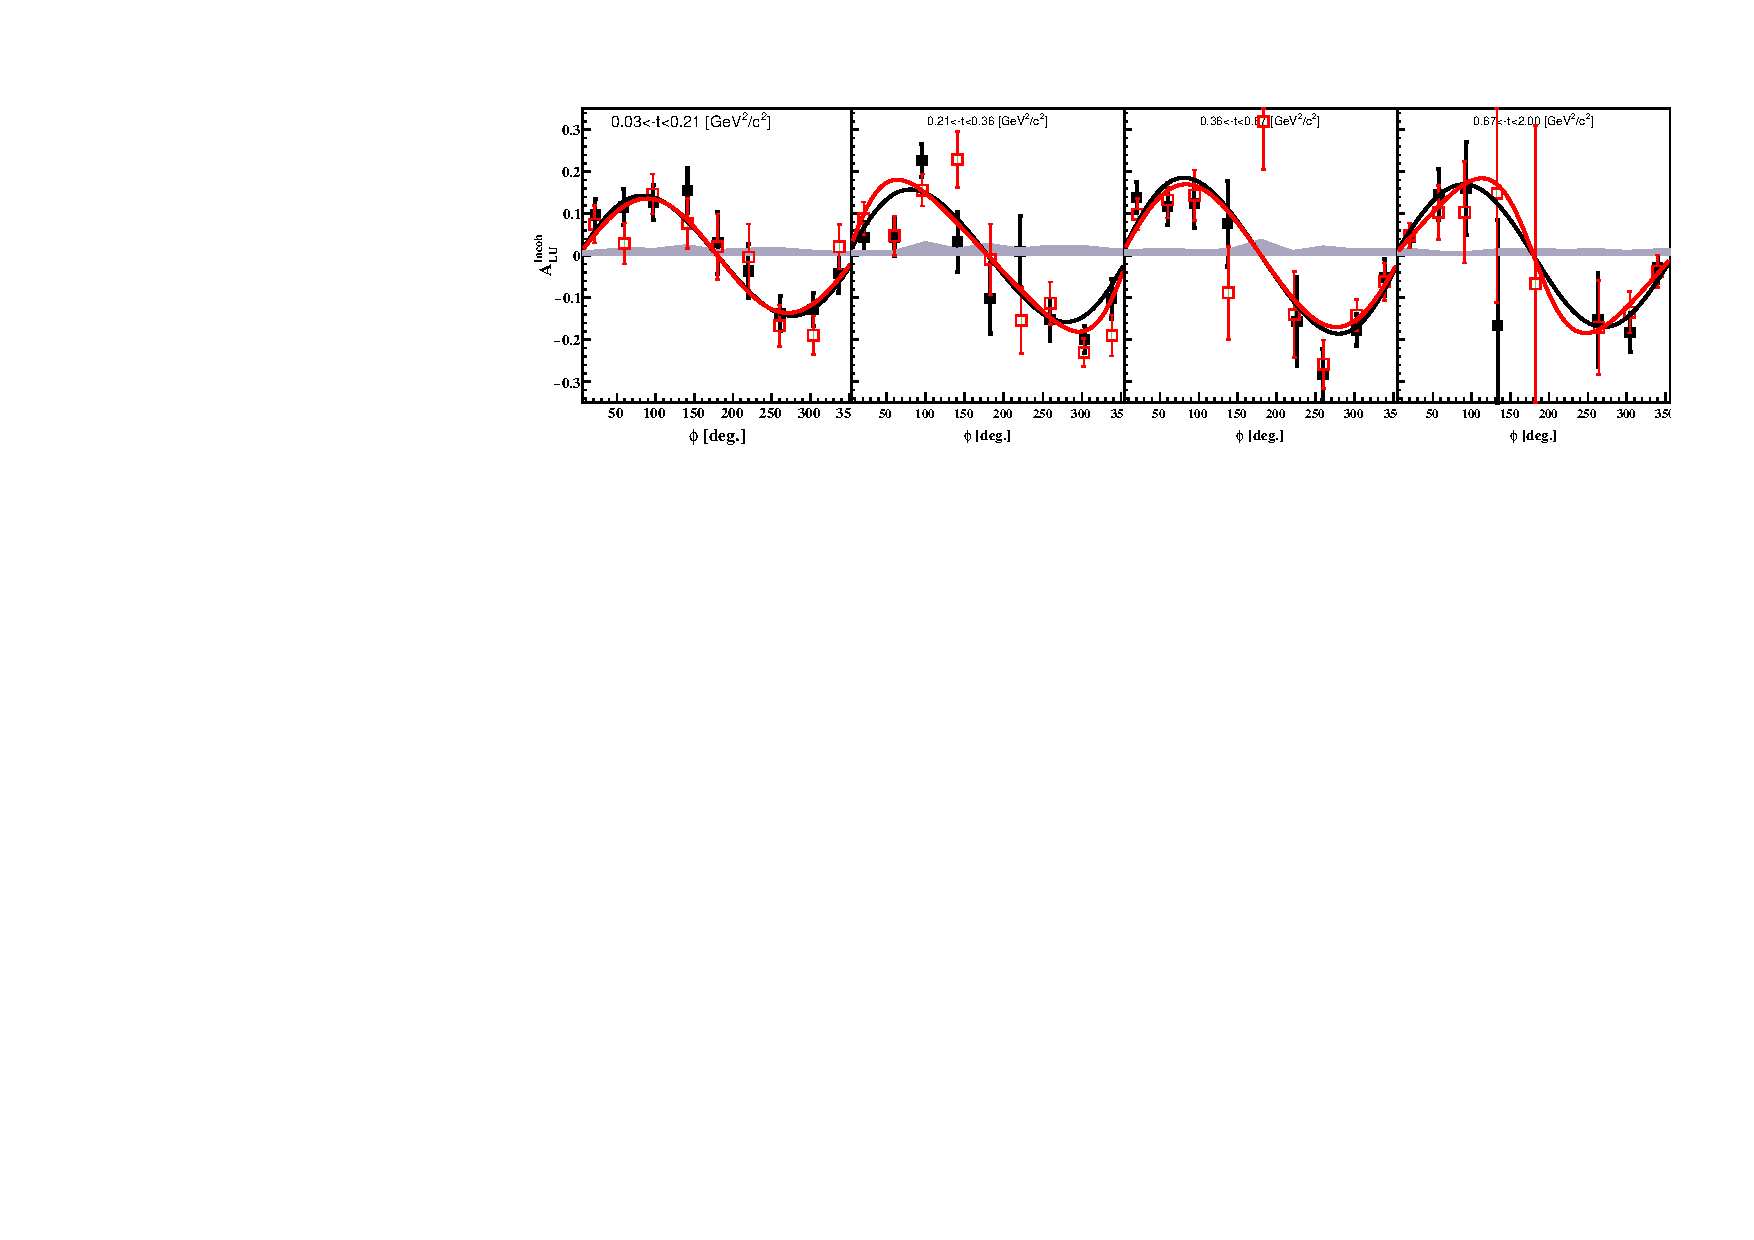
\includegraphics[height=6.0cm]{fig/ALU_phi_p_t.pdf}
\caption{The reconstructed incoherent $A_{LU}$ as a function of the angle 
   $\phi$ in $Q^2$, $x_B$, and $-t$ bins, respectively from top to bottom using 
$t$>$t_{min}$ in black squares, and $t'$>$t_{min}$ in red squares.}
   \label{fig:bsa_incoh_bins}
\end{figure}

\begin{figure}[h!]
   \centering
   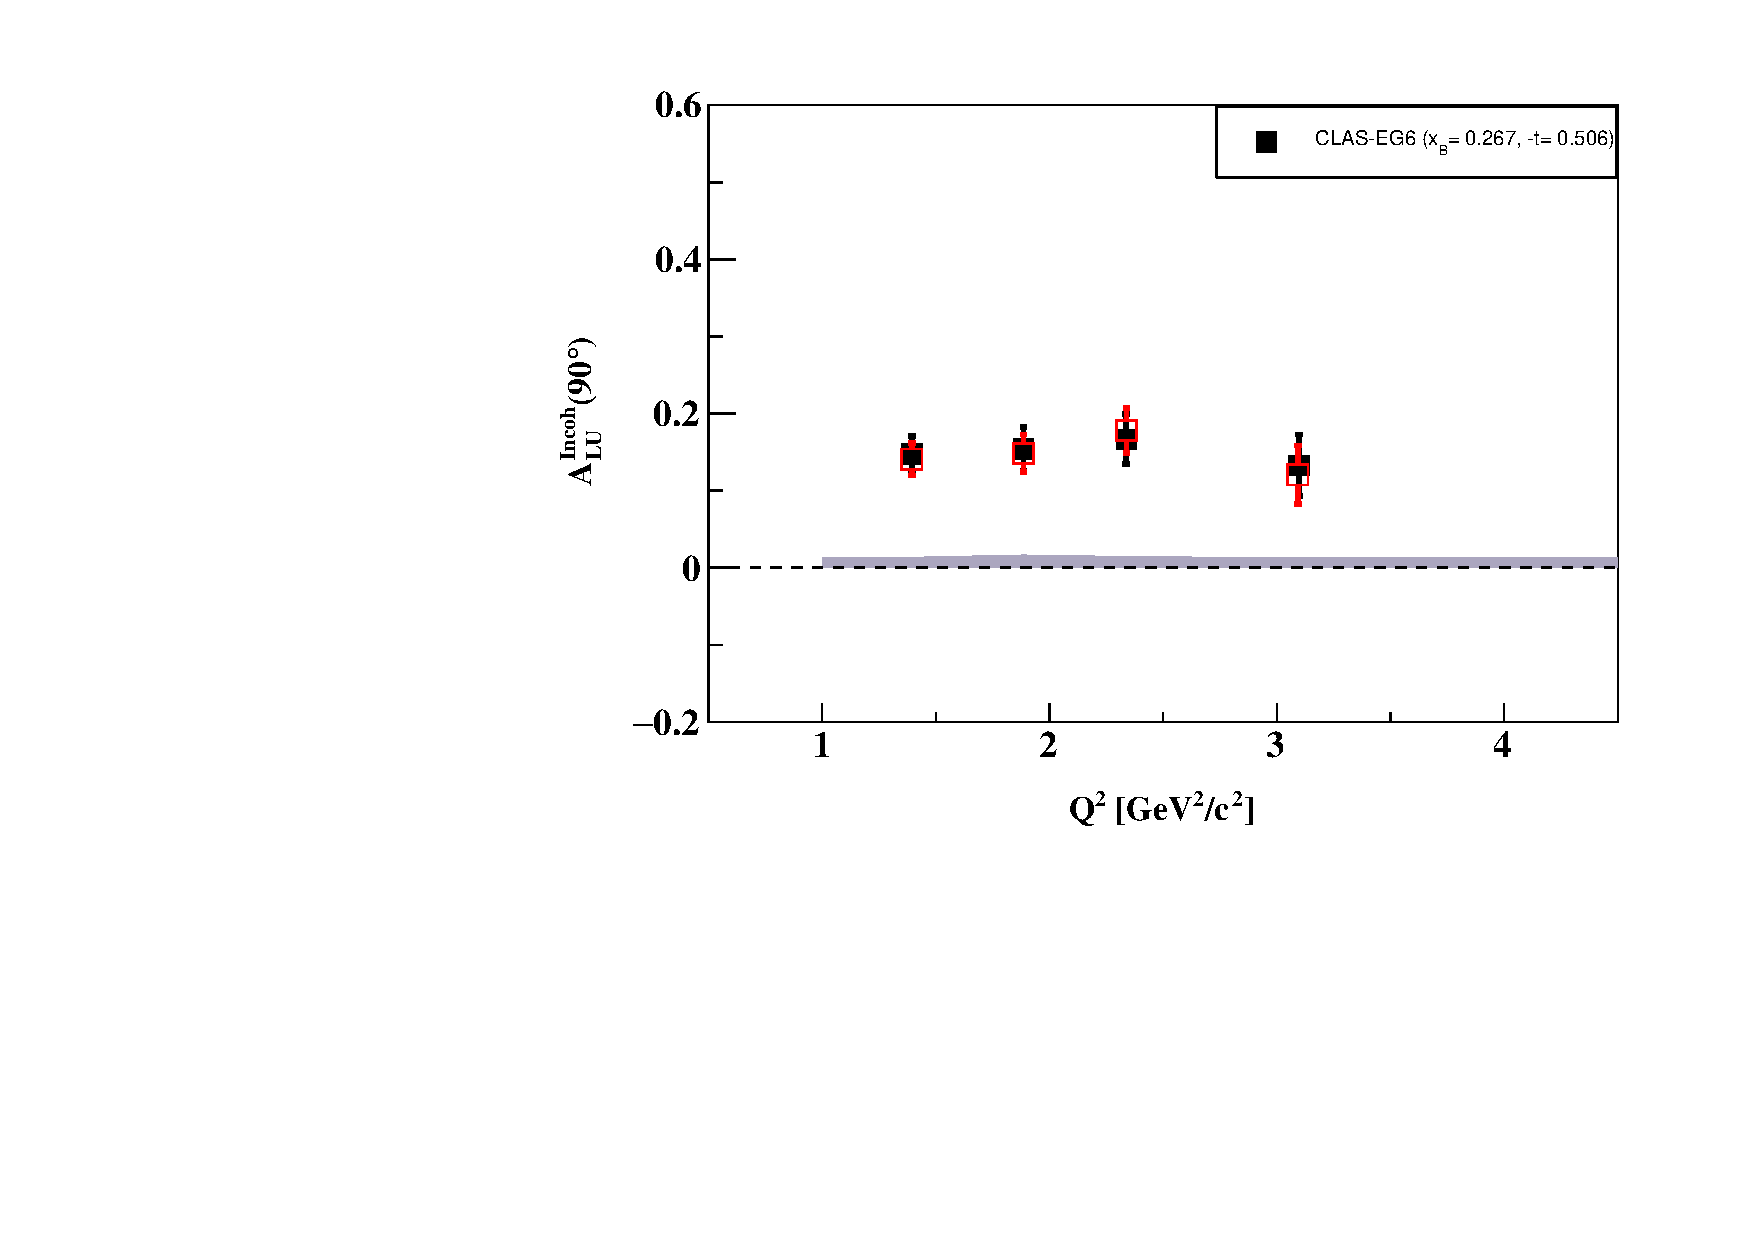
\includegraphics[height=6.0cm]{fig/ALU_90_p_vs_Q2_shortscenrario.pdf}\\
   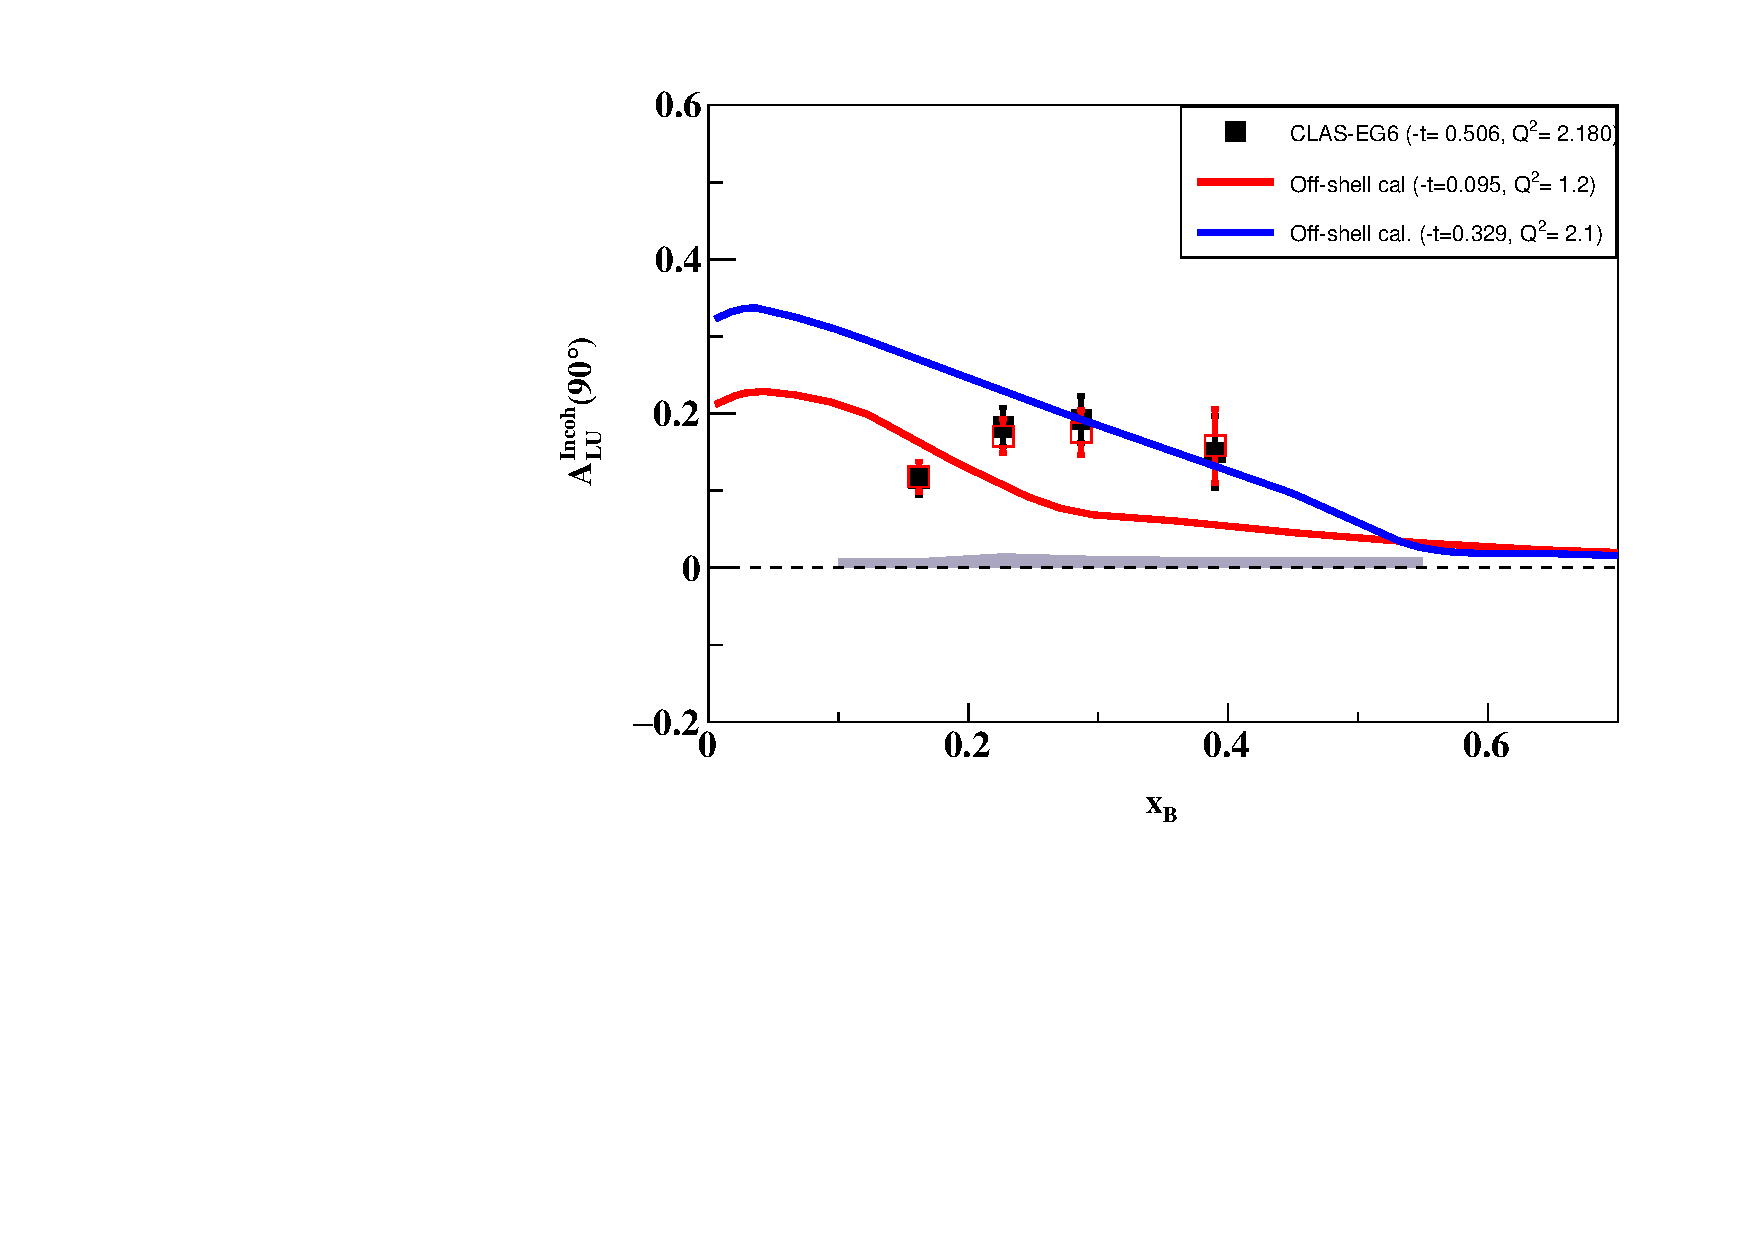
\includegraphics[height=6.0cm]{fig/ALU_90_p_vs_x_shortscenrario.pdf}\\
   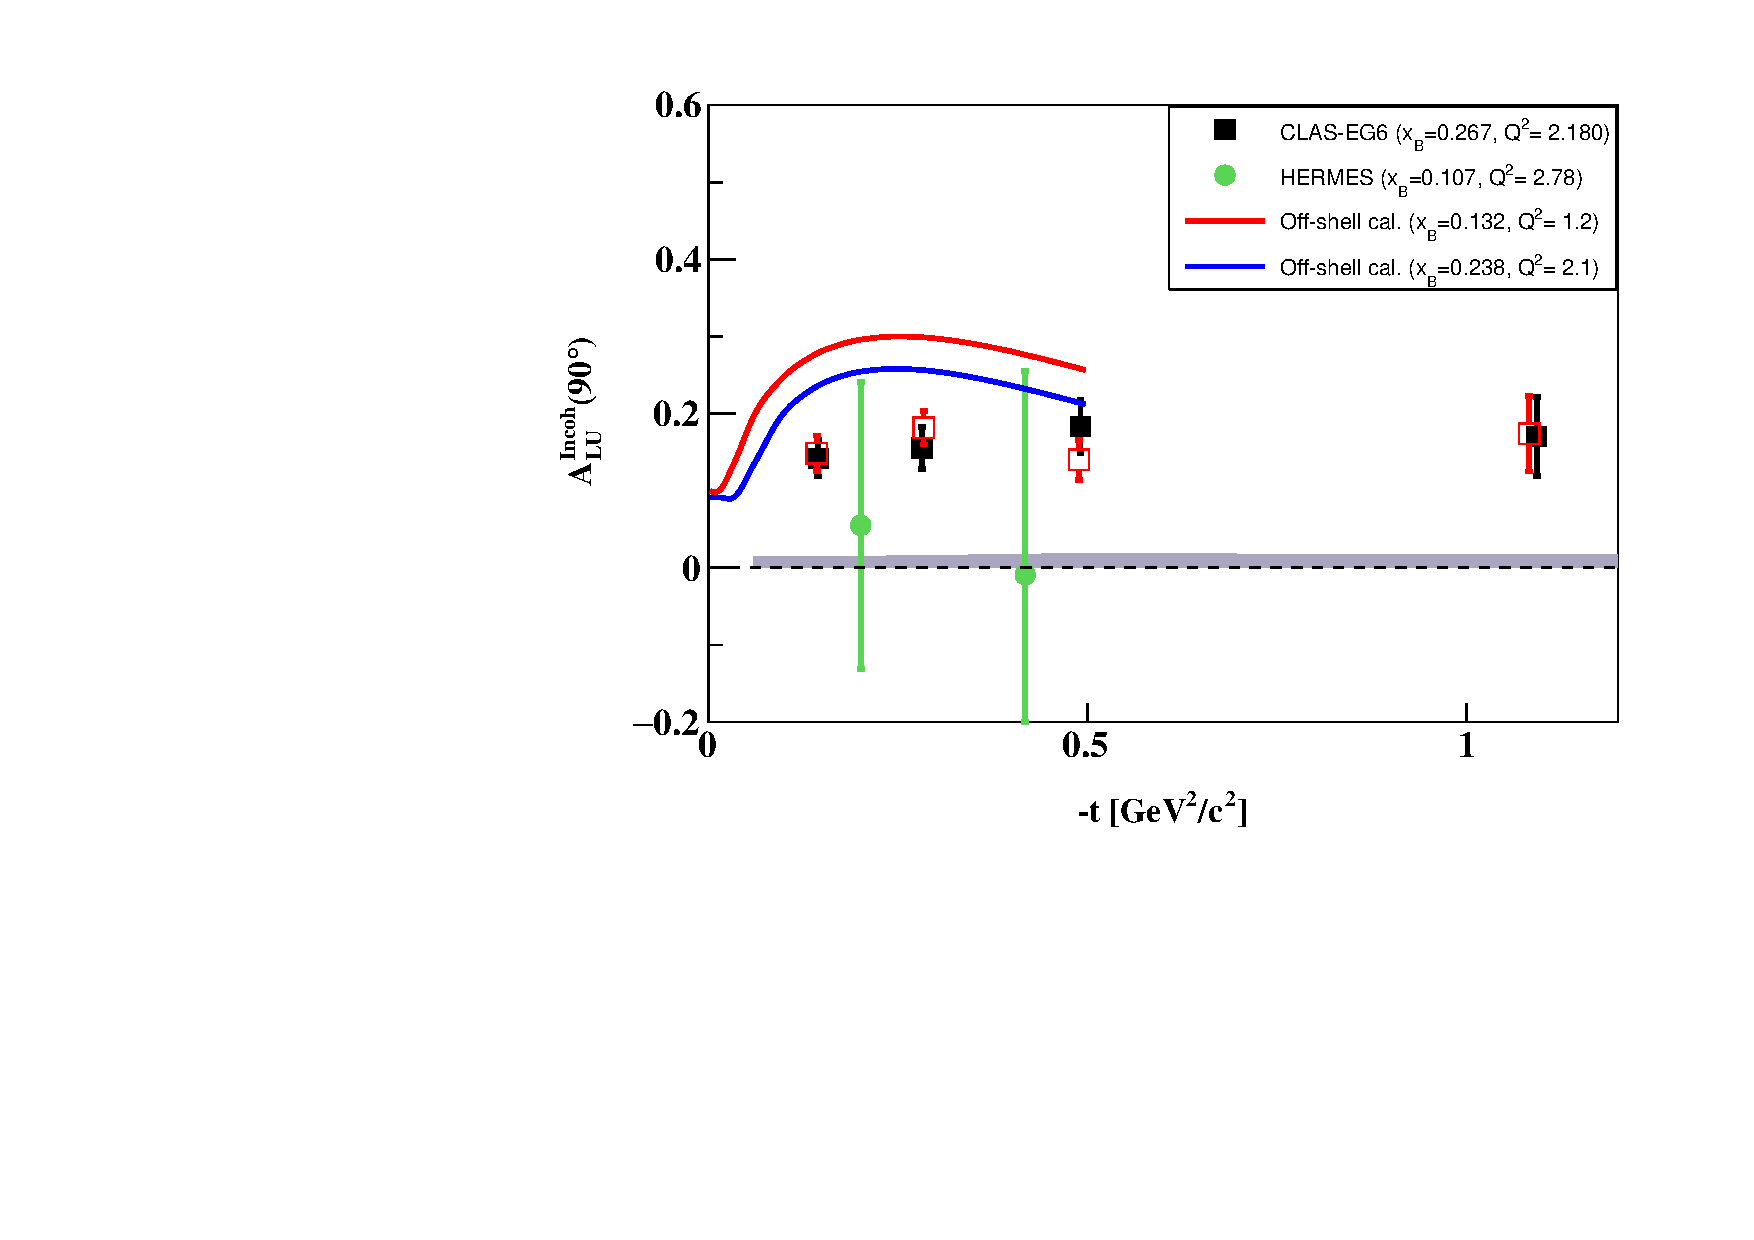
\includegraphics[height=6.0cm]{fig/ALU_90_p_vs_t_shortscenrario.pdf}
   \caption{The $Q^{2}$ (top), $x_{B}$ (middle), and $-t$-dependencies (bottom) 
      of the incoherent $A_{LU}$ at $\phi$~=~90$^{\circ}$, using the 
   $t$>$t_{min}$ cut and the corresponding exclusive cuts in black squares, and 
in red squares using the $t'$>$t_{min}$ and it's exclusive cuts.  The curves 
are theoretical calculations. On the bottom: the green circles are the HERMES 
$-A_{LU}$ (positron beam was used) inclusive measurements.}
\label{fig:incoh_Q2_xB_t_ALU}
\end{figure}



\section*{Conclusions}
In summary, we have studied the effects of Fermi motion on the measured 
incoherent beam-spin asymmetries by defining the transferred momentum squared 
through the nucleons in one case and through the photons in the other case. In 
terms of collected statistics, 2$\sigma$ exclusive cuts using the photons 
produced the same statistics as 3$\sigma$ cuts. The exclusive distributions 
using $t'$, through the photons, have shown more acceptable distributions in 
terms of being more symmetric in some cases and cleaner on others. The 
reconstructed asymmetries in the two cases of defining the transferred momentum 
squared are compatible and while the given error bars. As a suggestion, we 
would like to consider the $t'$ analysis as the final set for publications 
unless a major objections appear.



\end{document}
